\documentclass{article}
\usepackage{graphicx,float}
\usepackage{subfig}
\usepackage{geometry}
\geometry{a4paper}
\DeclareSubrefFormat{myparens}{#1-(#2)}
\captionsetup[subfloat]{subrefformat=myparens}


\begin{document}

\begin{figure}
	\def\CE{0.20}
	\centering
	\subfloat[]{
	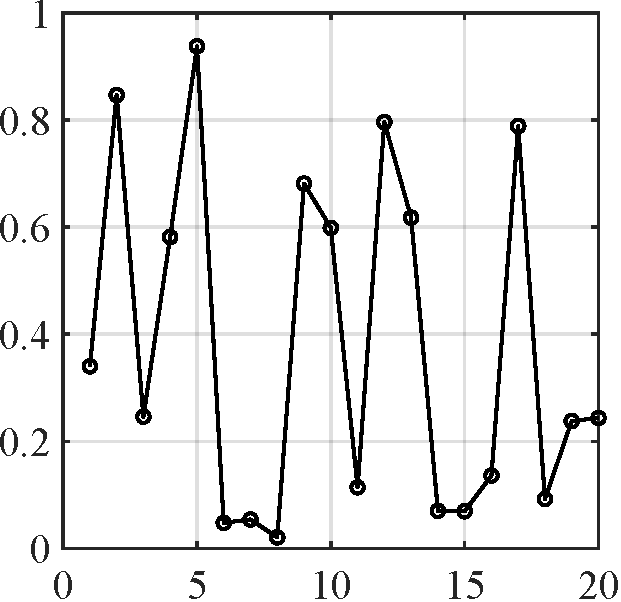
\includegraphics[height=\CE\textwidth, width=\CE\textwidth]{pic-1.pdf}
	\label{fig-a}}
	
	\subfloat[]{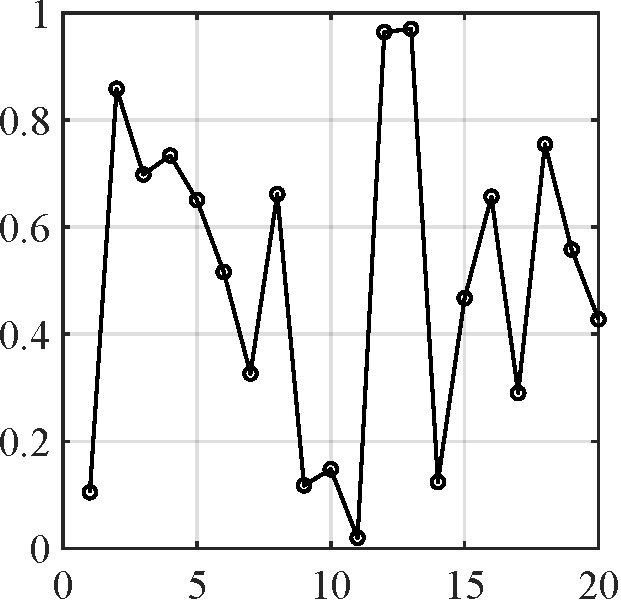
\includegraphics[height=\CE\textwidth, width=\CE\textwidth]{pic-2.pdf}}
	\caption{This is caption.}
	\label{fig}
\end{figure}

This is Fig. \ref{fig}, and this is subfigure Fig. \subref*{fig-a}.

\end{document}